	\subsection{UC1 - Web App - Autenticazione}
		
	\begin{figure}[H]
		\centering
		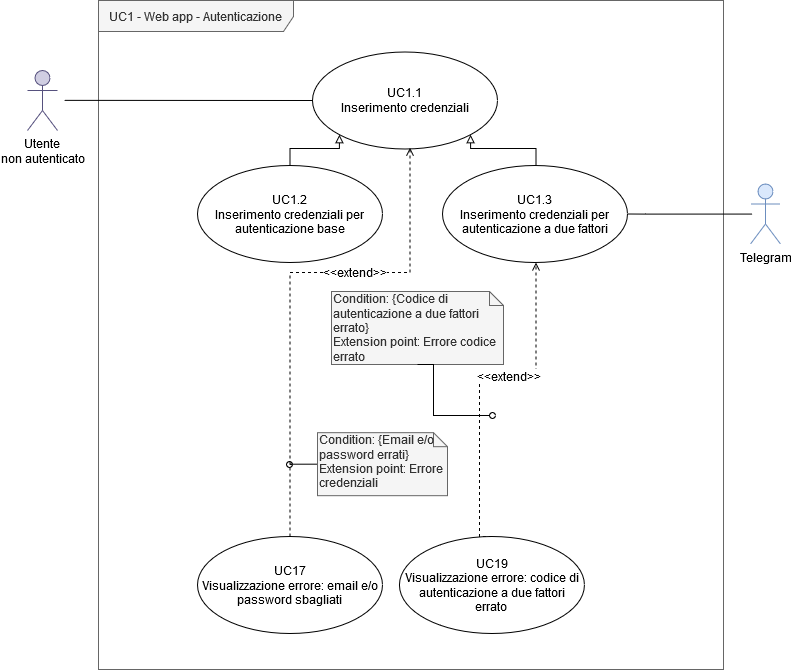
\includegraphics[scale=0.60]{res/images/uc1}
		\caption{Diagramma che riassume il processo di autenticazione nella web app.}
	\end{figure}
		
	\begin{itemize}
		\item \textbf{Attori Primari}: Utente non autenticato.
		\item \textbf{Attori Secondari}: \glock{Telegram}.
		\item \textbf{Descrizione}: L'utente vuole autenticarsi nella web app, per poter accedere alle funzionalità del sito.
		\item \textbf{Precondizione}: L'utente non è autenticato nella web app.
		\item \textbf{Postcondizione}: L'utente effettua l'autenticazione nella web app.
		\item \textbf{Scenario Principale}:
		\begin{enumerate}
			\item L'utente inserisce le proprie credenziali (UC 1.1);
			\item Viene eseguito il controllo delle credenziali inserite (UC 1.4).
		\end{enumerate}
	\end{itemize}
	

		\subsubsection{UC 1.1 - Inserimento credenziali}

		\begin{itemize}
			\item \textbf{Attori Primari}: Utente non autenticato.
			\item \textbf{Descrizione}: L'utente vuole autenticarsi nella web app e deve inserire alcuni campi obbligatori per procedere.
			\item \textbf{Precondizione}: L'utente non è autenticato nella web app.
			\item \textbf{Postcondizione}: L'utente ha inserito le credenziali richieste.
			\item \textbf{Scenario Principale}:
			\begin{enumerate}
				\item L'utente inserisce le credenziali per l'autenticazione base (UC 1.2);
				\item L'utente inserisce le credenziali per l'autenticazione a due fattori (UC 1.3);
			\end{enumerate}
			\item \textbf{Inclusioni}:
				\begin{itemize}
					\item Controllo credenziali (UC 1.4).
				\end{itemize}
			\item \textbf{Estensioni}:
				\begin{itemize}
					\item Visualizzazione errore: email e/o una password errati (UC 17).
				\end{itemize}
		\end{itemize}

		\subsubsection{UC 1.2 - Inserimento credenziali per autenticazione base}

		\begin{figure}[H]
			\centering
			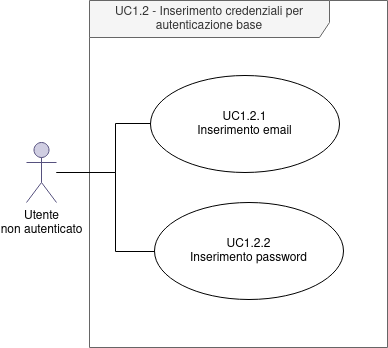
\includegraphics[scale=0.675]{res/images/uc1.2}
			\caption{Diagramma che descrive l'inserimento delle credenziali per l'autenticazione base.}
		\end{figure}

		\begin{itemize}
			\item \textbf{Attori Primari}: Utente non autenticato.
			\item \textbf{Descrizione}: L'utente vuole autenticarsi nella web app ed inserisce i campi obbligatori per l'autenticazione base.
			\item \textbf{Precondizione}: L'utente non è autenticato nella web app.
			\item \textbf{Postcondizione}: L'utente ha inserito le credenziali richieste.
			\item \textbf{Scenario Principale}:
			\begin{enumerate}
				\item L'utente inserisce la email (UC 1.2.1);
				\item L'utente inserisce la password (UC 1.2.2).
			\end{enumerate}	
		\end{itemize}

			\paragraph{UC 1.2.1 - Inserimento email}
			\begin{itemize}
				\item \textbf{Attori Primari}: Utente non autenticato.
				\item \textbf{Descrizione}: L'utente vuole autenticarsi nella web app e inserisce uno dei campi obbligatori per l'autenticazione base.
				\item \textbf{Precondizione}: L'utente non è autenticato nella web app.
				\item \textbf{Postcondizione}: L'utente ha inserito la credenziale richiesta.
				\item \textbf{Scenario Principale}:
				\begin{enumerate}
					\item L'utente compila il campo email.
				\end{enumerate}	
			\end{itemize}

			\paragraph{UC 1.2.2 - Inserimento password}
			\begin{itemize}
				\item \textbf{Attori Primari}: Utente non autenticato.
				\item \textbf{Descrizione}: L'utente vuole autenticarsi nella web app e inserisce uno dei campi obbligatori per l'autenticazione base.
				\item \textbf{Precondizione}: L'utente non è autenticato nella web app.
				\item \textbf{Postcondizione}: L'utente ha inserito la credenziale richiesta.
				\item \textbf{Scenario Principale}:
				\begin{enumerate}
					\item L'utente compila il campo password.
				\end{enumerate}	
			\end{itemize}

		\subsubsection{UC 1.3 - Inserimento credenziali per autenticazione a due fattori}

		\begin{figure}[H]
			\centering
			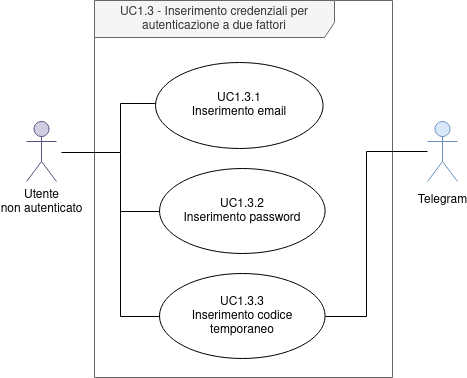
\includegraphics[scale=0.675]{res/images/uc1.3}
			\caption{Diagramma che descrive l'inserimento delle credenziali per l'autenticazione a due fattori.}
		\end{figure}

		\begin{itemize}
			\item \textbf{Attori Primari}: Utente non autenticato.
			\item \textbf{Attori Secondari}: \glock{Telegram}.
			\item \textbf{Descrizione}: L'utente vuole autenticarsi nella web app ed inserisce i campi obbligatori per l'autenticazione a due fattori.
			\item \textbf{Precondizione}: L'utente non è autenticato nella web app.
			\item \textbf{Postcondizione}: L'utente ha inserito le credenziali richieste.
			\item \textbf{Scenario Principale}:
				\begin{enumerate}
					\item L'utente inserisce la email (UC 1.3.1);
					\item L'utente inserisce la password (UC 1.3.2);
					\item L'utente inserisce un codice temporaneo ricevuto tramite \glock{Telegram} (UC 1.3.3).
				\end{enumerate}
			\item \textbf{Estensioni}:
				\begin{itemize}
					\item Visualizzazione errore: codice di autenticazione a due fattori errato (UC 19).
				\end{itemize}	
		\end{itemize}

			\paragraph{UC 1.3.1 - Inserimento email}
			\begin{itemize}
				\item \textbf{Attori Primari}: Utente non autenticato.
				\item \textbf{Descrizione}: L'utente vuole autenticarsi nella web app e inserisce uno dei campi obbligatori per l'autenticazione a due fattori.
				\item \textbf{Precondizione}: L'utente non è autenticato nella web app.
				\item \textbf{Postcondizione}: L'utente ha inserito la credenziale richiesta.
				\item \textbf{Scenario Principale}:
				\begin{enumerate}
					\item L'utente compila il campo email.
				\end{enumerate}	
			\end{itemize}

			\paragraph{UC 1.3.2 - Inserimento password}
			\begin{itemize}
				\item \textbf{Attori Primari}: Utente non autenticato.
				\item \textbf{Descrizione}: L'utente vuole autenticarsi nella web app e inserisce uno dei campi obbligatori per l'autenticazione a due fattori.
				\item \textbf{Precondizione}: L'utente non è autenticato nella web app.
				\item \textbf{Postcondizione}: L'utente ha inserito la credenziale richiesta.
				\item \textbf{Scenario Principale}:
				\begin{enumerate}
					\item L'utente compila il campo password.
				\end{enumerate}	
			\end{itemize}

			\paragraph{UC 1.3.3 - Inserimento codice temporaneo}
			\begin{itemize}
				\item \textbf{Attori Primari}: Utente non autenticato.
				\item \textbf{Attori Secondari}: \glock{Telegram}.
				\item \textbf{Descrizione}: L'utente vuole autenticarsi nella web app e inserisce uno dei campi obbligatori per l'autenticazione a due fattori.
				\item \textbf{Precondizione}: L'utente non è autenticato nella web app.
				\item \textbf{Postcondizione}: L'utente ha inserito la credenziale richiesta.
				\item \textbf{Scenario Principale}:
				\begin{enumerate}
					\item L'utente riceve una notifica tramite \glock{Telegram} con un codice temporaneo;
					\item L'utente compila il campo codice temporaneo.
				\end{enumerate}	
			\end{itemize}

		\subsubsection{UC 1.4 - Controllo credenziali}
		\begin{itemize}
			\item \textbf{Attori Primari}: Utente non autenticato.
			\item \textbf{Descrizione}: L'utente vuole autenticarsi nella web app e il sistema controlla che le credenziali inserite siano valide.
			\item \textbf{Precondizione}: L'utente non è autenticato nella web app e ha inserito le credenziali richieste.
			\item \textbf{Postcondizione}: L'utente ha inserito delle credenziali valide ed effettua l'autenticazione.
			\item \textbf{Scenario Principale}:
			\begin{enumerate}
				\item L'utente ha inserito le credenziali richieste;
				\item Le credenziali inserite vengono controllate dal sistema.
			\end{enumerate}
			\item \textbf{Estensioni}:
			\begin{itemize}
				\item Visualizzazione errore: l'account non è autorizzato (UC 18).
			\end{itemize}	
		\end{itemize}
